\documentclass{article}
\usepackage{graphicx} % Required for inserting images
\usepackage{caption}
\usepackage{subcaption}
\usepackage{geometry}
\usepackage[x11names]{xcolor}
\usepackage{listings}
\usepackage{minted}
\usepackage{xparse}
\usepackage{wrapfig}
\usepackage{amsmath}
\usepackage{float}
\usepackage{xcolor}
\usepackage[
    backend=biber,
    style=alphabetic,
    sorting=ynt
]{biblatex}
\usepackage{hyperref}
\addbibresource{references.bib}

\hypersetup{
    colorlinks=true,
    linkcolor=blue,
    citecolor=SpringGreen4,
    filecolor=magenta,      
    urlcolor=cyan,
    pdftitle={Application of Multithreading to the Floyd-Steinberg Dithering Algorithm},
    pdfpagemode=FullScreen,
    }

\definecolor{shellbackground}{rgb}{0.95,0.95,0.92}

\geometry{
a4paper,
margin=0.75in,
top=0.65in
}

\title{Application of Multithreading to the Floyd-Steinberg Dithering Algorithm for Image Manipulation}
\author{Ashish Thomas Mathew}
\date{}

\begin{document}

\maketitle
\begin{abstract}
    \noindent Dithering is a noise-introduction method that is widely used in various fields ranging from the optimization of graphics in videogames to newspaper printing. With the increasing quality and resolution of images and video, including gigapixel resolutions, it would be interesting to see how parallel processing could be implemented in the process of dithering. We will be looking into Floyd-Steinberg Dithering, an error-diffusion image dithering algorithm designed and published by Robert W. Floyd and Louis Steinberg in 1976, and the challenges faced in the the application of multithreaded processing to it.  
\end{abstract}

\section{Introduction}\label{Introduction}

We have seen a great deal of development in digital media in today's world, especially in the field of image processing, where the quality of images generated has increased with resolutions ranging from a few thousand to several millions of pixels. Consequently, we have also seen several solutions to handling these images when using hardware with low specifications. One of the main solutions used is \textbf{dithering}. In this project we will be looking into dithering algorithms, specifically the Floyd-Steinberg dithering algorithm\cite{Steinberg} in the context of High-Performance Computing to deduce whether parallelized processing would be an effective way to improve its performance on large images.

\subsection{What is Dithering?}\label{Dithering Intro}

Dithering is the process of deliberately introducing noise into data to prevent the formation of fixed patterns or distortion. Some examples of these distortions are unwanted high or low frequency disturbances in audio signals and the formation of color bands when images are compressed. Dithering randomizes the patterns formed to help avoid the generation of anomalous artifacts in the given piece of media.

\medskip
\noindent In computer graphics, dithering is used to simulate shading by approximating the colors present in an image, to help improve its quality and reduce the artifacts that could be introduced into it when downscaling it. This is particularly useful when we have images with a large range of colors than the display hardware can handle. There have been several dithering algorithms developed that try to achieve this, such as

\begin{itemize}
    \item \textit{Average Dithering}, also known as \textit{quantization}, which is a dithering method where, for each pixel the value of the color channels are determined by an average threshold value.

    \item \textit{Ordered Dithering} which makes use of a threshold map matrix to change the color of pixels depending on how far the original color is from a reduced palette.

    \item \textit{Error Diffusion Dithering}, which is a method of dithering that involves quantizing the value of a given pixel and distributing the error of the current pixel's RGB color channels to the neighboring pixels.

    \item \textit{Physical models} such as Lattice-Boltzmann Dithering\cite{Hagenburg}.

\end{itemize}

\medskip
\noindent One of the most well known image dithering algorithms is Floyd-Steinberg Dithering\cite{Steinberg}. What sets this algorithm apart from the others mentioned here is that the images generated by it have a quality closest to the original image while also effectively reducing its color palette.

\medskip
\noindent Given that the working of this algorithm is based on error diffusion, the process of parallelizing it is not as simple as just dividing up the work between threads and executing the program, which would normally be the case for an embarrassingly parallel problem. This is because every pixel has a strong dependency on the pixels around it. We will be looking into developing an approach to solving this problem in this project.

\section{The Floyd-Steinberg Dithering Algorithm}\label{Floyd-Steinberg Dithering}

Most error diffusion algorithms work on the same principle\cite{computerphile} of reducing the number of bits we need to represent in each of the colors, and then implementing a pixel-by-pixel spread of the error from the given pixel to its neighbors to simulate the transition between the various colors present in the image. The main difference is in the value of error being propagated to the neighboring pixels.

\medskip
\noindent For a given image, consider the fact that every pixel present in the image has a color value that is composed of three main channels, \textcolor{red}{Red}, \textcolor{Green4}{Green} and \textcolor{blue}{Blue}, each having ranges between 0 to 255, that is, each having 256 ($2^8$) possible shades. We could represent a pixel at a given position as

 \begin{equation} 
    \text{Pixel}(y,x) = (\underbrace{0\to255}_\text{Blue Channel},\underbrace{0\to255}_\text{Green Channel},\underbrace{0\to255}_\text{Red Channel})\label{Pixel Values}
 \end{equation}

\noindent where $(y,x)$ represents the position of the particular pixel starting from the top-left corner of the image, with \textbf{y representing each column of pixels and x representing each row of pixels}. If we were to consider the possible number of colors a pixel can have from (\ref{Pixel Values}), it\ would be

$$\text{Number of Possible colors} = 2^8\times2^8\times2^8 = 16,777,216$$

\noindent which is a very large number of possible colors that an image could have. If we were to reduce the possible number of colors per channel to, say, 2 colors, that is, either 0 or 255 for each color channel, we would get the total number of possible colors per image to be 

$$\text{Number of Possible colors} = 2\times2\times2 = 8$$

\noindent which is much lesser. However, as a consequence, we notice distinct color banding in the resultant image, making it obvious to see that its quality has degraded. This is where the error diffusion comes into the picture.

\medskip

\begin{figure}[H]
  \centering
  \begin{subfigure}[t]{0.35\textwidth}
    \centering
    
\includegraphics[width=\textwidth]{images/me.jpg}
    \caption{A picture of me}
    \label{fig:me}
  \end{subfigure}
  ~
  \begin{subfigure}[t]{0.35\textwidth}
    \centering
    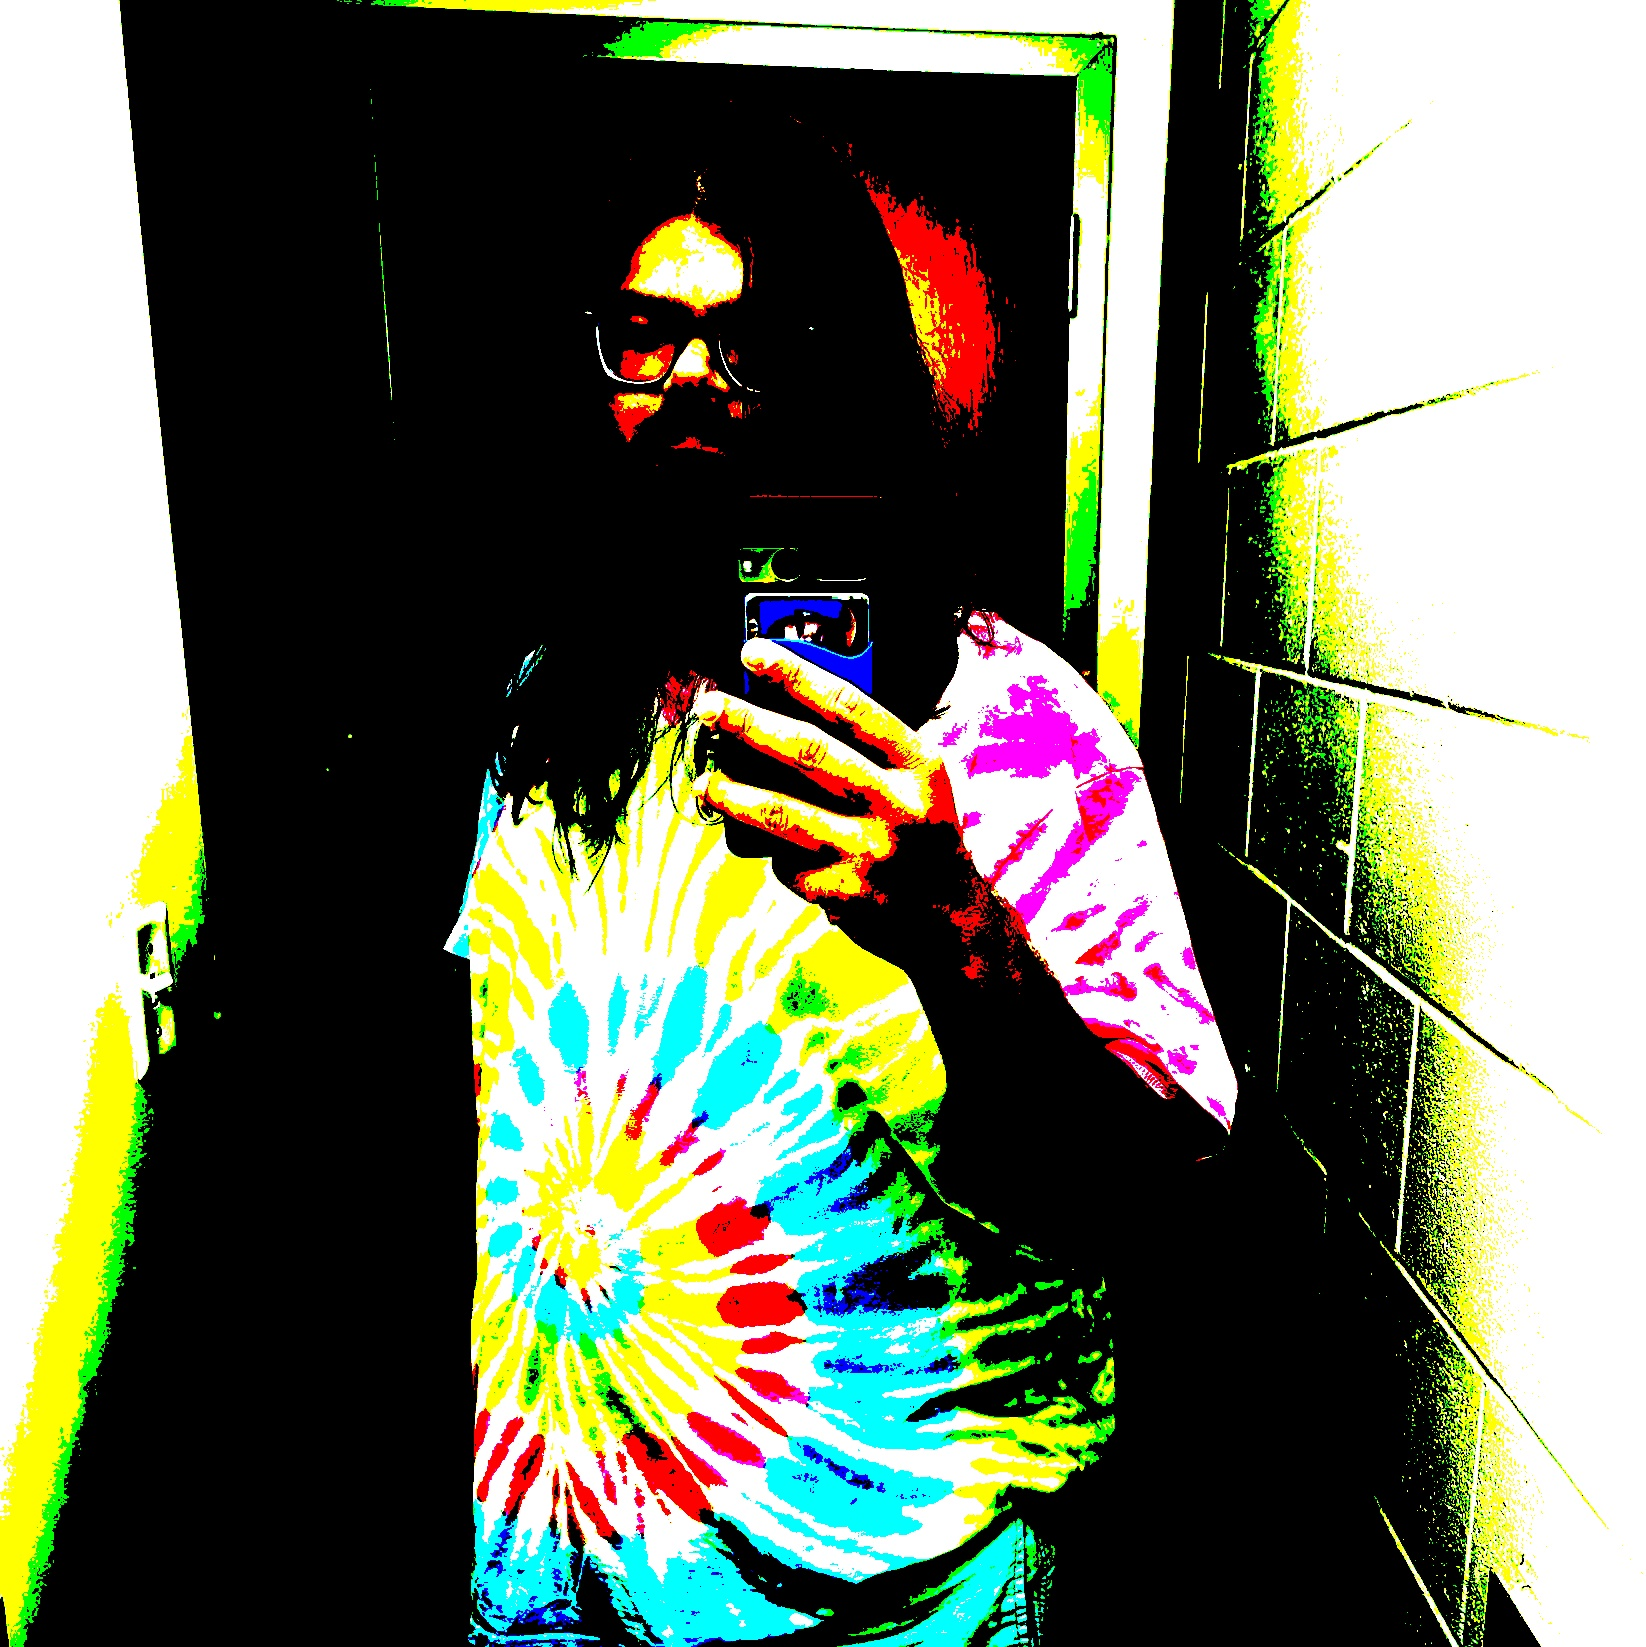
\includegraphics[width=\textwidth]{images/quantized_me.jpg}
    \caption{Me, but quantized to a factor of 1}
    \label{fig:me_quantized}
  \end{subfigure}
  \caption{An example of how quantization leads to banding in images}
\end{figure}

\noindent Instead of moving on to the next pixel directly after quantizing the current pixel, we would diffuse the error with the following steps\cite{guilloteau:hal}

\begin{enumerate}
    \item Take the current pixel and generate a new color value for it based on a threshold \textit{factor}. For a factor of 1, the threshold would be the midway point, leading to two possible values per channel, either 0 or 255. Similarly, for a factor of 2, we would have 3 different possible colors, and so on.

    \item Find the error between the original BGR color value of the given pixel and the newly found quantized value. We take this to be the \textit{quantization error}.

    \item We then take this error, split it up into fractions, and distribute each part to the neighboring pixels.
\end{enumerate}

\noindent This process is then repeated at every pixel until we achieve a good amount of distribution of the error across the whole image, hence reducing the banding to a significant extent.

\begin{figure}[H]
    \centering
    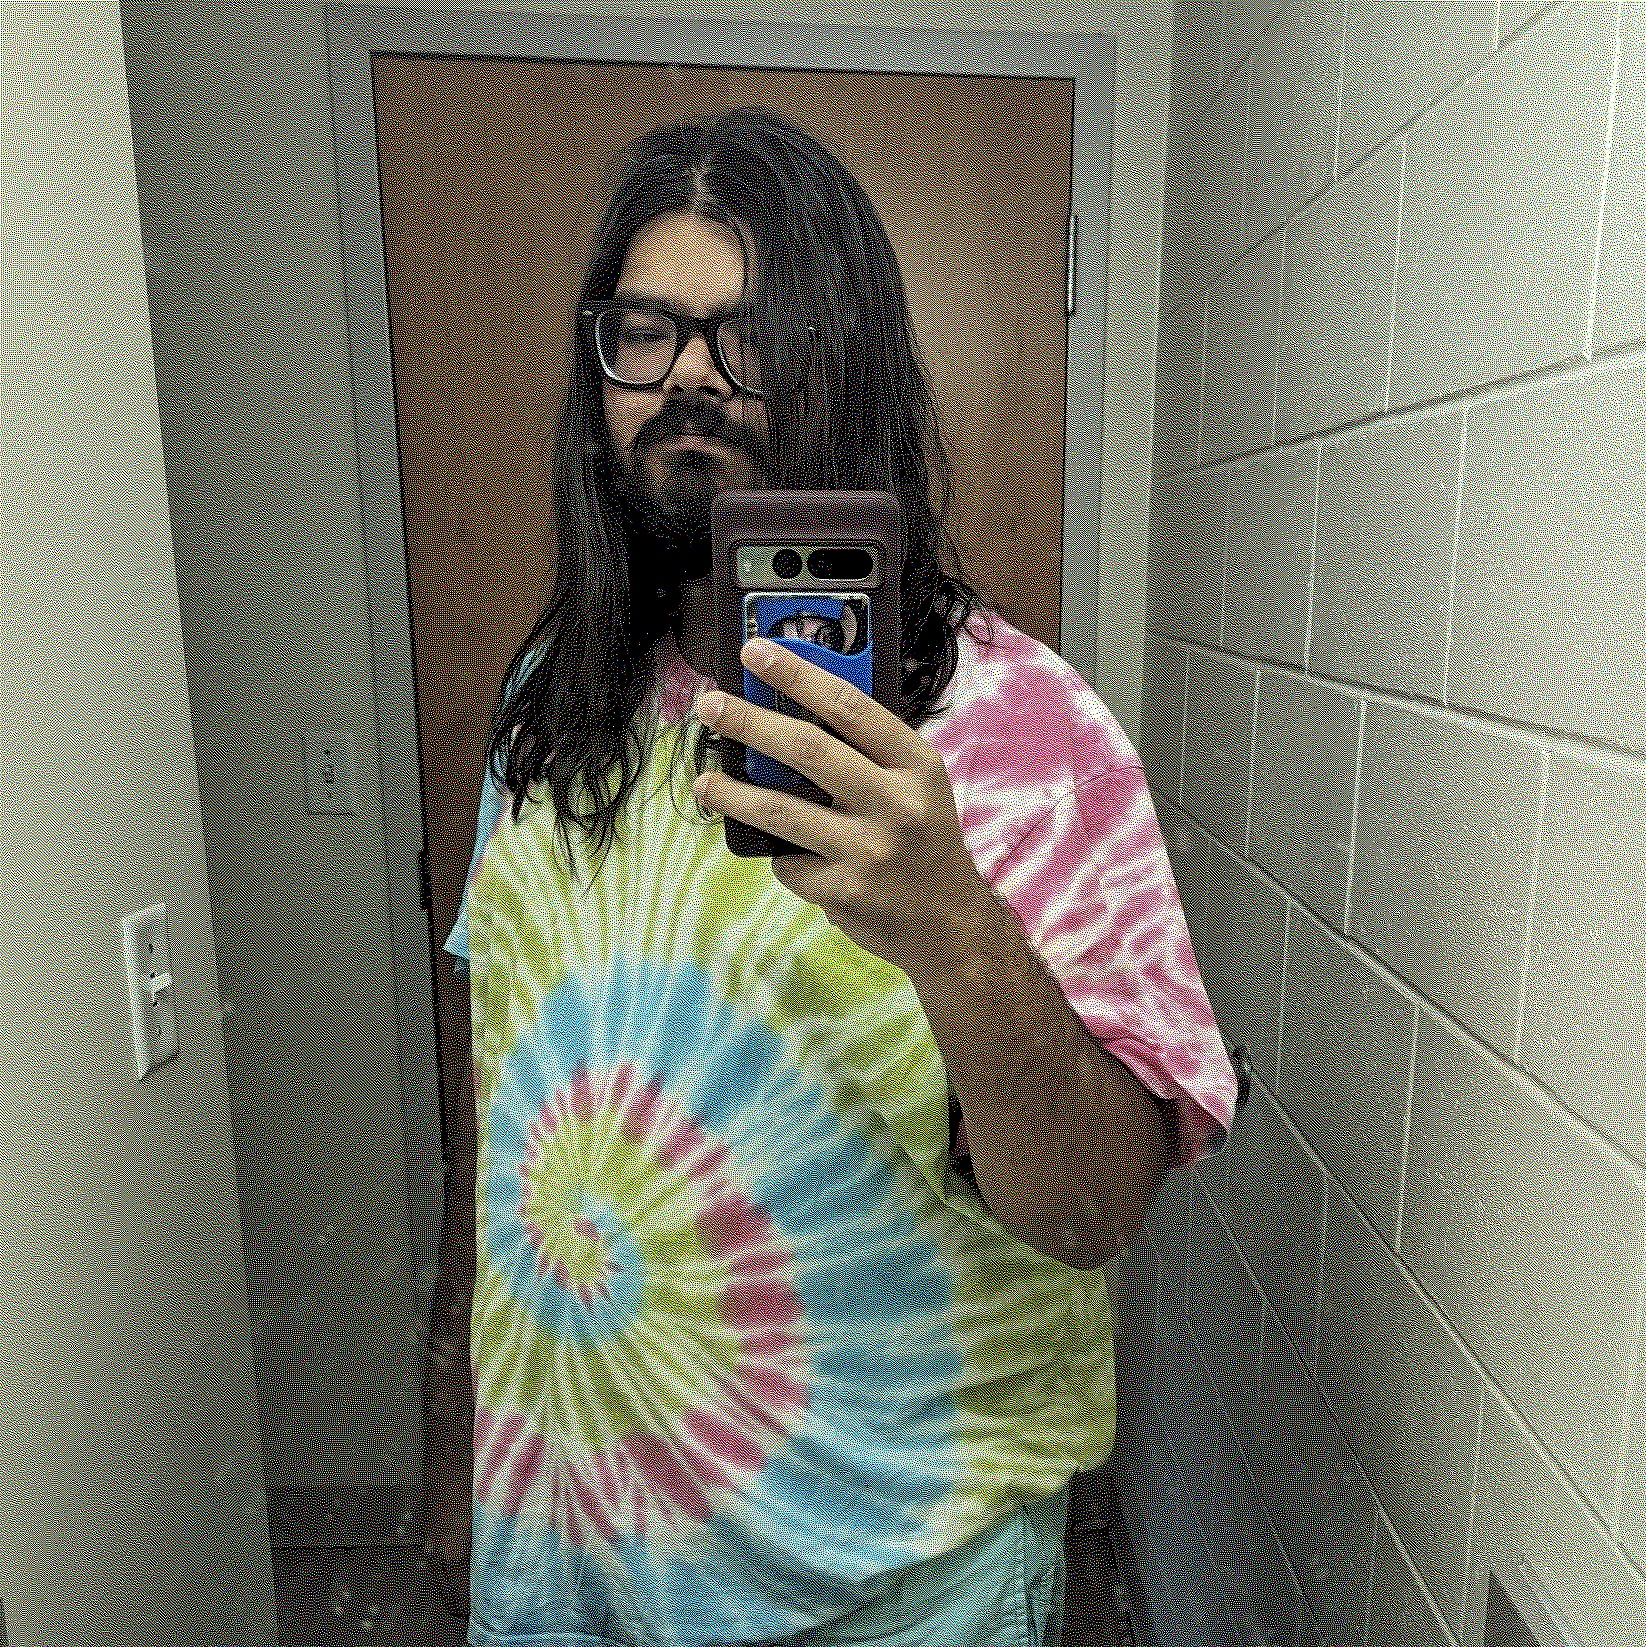
\includegraphics[width=0.35\textwidth]{images/dithered_me.jpg}
    \caption{A picture of me after dithering at the same quantization factor of 1}
    \label{fig:me_dithered}
\end{figure}

\subsection{Mechanism of the Algorithm}\label{Floyd-Steinberg Mechanism}

\noindent In all the error diffusion methods, the mechanism of the algorithm is, for the most part, the same. The only thing that varies is the numerical constants that represent the fractions that we are distributing to the neighboring pixels\cite{guilloteau:hal}.

\medskip

\noindent In the case of the Floyd-Steinberg dithering algorithm, the current pixel being worked on is first quantized, after which, the adjacent pixels receive the error from the current pixel as follows

\medskip
\renewcommand{\arraystretch}{1.5}
$$
    \begin{bmatrix}
        *   &      *      &      X      & \frac{7}{16} & \dots \\
      \dots & \frac{3}{16} & \frac{5}{16} & \frac{1}{16} & \dots \\
     
    \end{bmatrix} \qquad
    \text{\parbox{7cm}{where X represents the current pixel being worked on and * represents pixels that have already been worked on }}
$$

\medskip
\noindent Suppose we have a pixel

$$\text{Pixel}(y,x) = (85,155,0)$$

\noindent Upon quantizing this pixel at a factor of 1, we get the quantized pixel and the corresponding error as

\begin{align*}
\text{Pixel}_Q(y,x) &= (0,255,0) \\
\text{Error}(y,x) &= (85,-100,0)
\end{align*}

\noindent This error is then spread out to the neighboring pixels such that

\medskip
\noindent for the pixel to the right of the current pixel:

$$
    \text{Pixel}(y+1,x) = \left(\left(b+\left(\frac{7}{16}\times(85)\right)\right),\left(g+\left(\frac{7}{16}\times(-100)\right)\right),\left(r+\left(\frac{7}{16}\times(0)\right)\right)\right)  
$$

\noindent for the pixel to the bottom right of the current pixel:

$$
    \text{Pixel}(y+1,x+1) = \left(\left(b+\left(\frac{1}{16}\times(85)\right)\right),\left(g+\left(\frac{1}{16}\times(-100)\right)\right),\left(r+\left(\frac{1}{16}\times(0)\right)\right)\right)
$$

\noindent for the pixel below the current pixel:

$$
    \text{Pixel}(y,x+1) = \left(\left(b+\left(\frac{5}{16}\times85)\right)\right),\left(g+\left(\frac{5}{16}\times(-100)\right)\right),\left(r+\left(\frac{5}{16}\times(0)\right)\right)\right)
$$

\noindent and finally for the pixel to the bottom left of the current pixel:

$$
    \text{Pixel}(y+1,x-1) = \left(\left(b+\left(\frac{3}{16}\times(85)\right)\right),\left(g+\left(\frac{3}{16}\times(-100)\right)\right),\left(r+\left(\frac{3}{16}\times(0)\right)\right)\right)
$$

\noindent where $b$, $g$ and $r$ represent the blue, green and red color channel values respectively. We repeat this process while moving from left to right along the same row and then moving on to the next row once the current one is completed. In the case of the current pixel being at any of the edges of the image, there would be no need to propagate the error past the edge.

\subsection{Pseudocode for the Algorithm}\label{Floyd-Steinberg Pseudocode}

The implementation of the above algorithm in code would look like

\begin{minted}[
frame=lines,
framesep=2mm,
baselinestretch=1.2,
bgcolor=Cornsilk2,
fontsize=\footnotesize,
linenos
]{Python}
factor = # An integer factor determined by the user
for each row from top to bottom:
    for each column from left to right:
        oldpixel = image[column][row]

        # Quantizing the current pixel and calculating the error
        newpixel = quantize(oldpixel, factor)
        image[column][row] = newpixel
        quantization_error = oldpixel - newpixel

        # Spreading the quantization error to the surrounding pixels
        image[column+1][row]   = clamp(image[column+1][row]   + (quantization_error*7/16))
        image[column+1][row+1] = clamp(image[column+1][row+1] + (quantization_error*1/16))
        image[column][row+1]   = clamp(image[column][row+1]   + (quantization_error*5/16))
        image[column+1][row-1] = clamp(image[column+1][row-1] + (quantization_error*3/16))

function quantize(pixel, factor):
    return round(factor * pixel/255.0) * 255/factor

# This function prevents the color values from going above 255 or below 0
function clamp(value):
    return max(0, min(value, 255))
\end{minted}

\noindent \textbf{For our use case, we will be keeping the quantization factor fixed at 1 for all upcoming runs of the code}

\section{Implementing the Floyd-Steinberg Dithering Algorithm}\label{Implementing Floyd-Steinberg Dithering}

We implement the pseudocode in section [\ref{Floyd-Steinberg Pseudocode}] in C++ using OpenCV to access and manipulate the pixel information of the image. The following observations were made on two test images:

\begin{itemize}
    \item Processing a small test image of 512x512 dimensions takes, on average, 0.0965 seconds.

    \item Processing a large test image of 7680x4320 dimensions takes, on average, 11.07 seconds.
\end{itemize}

\section{Parallelizing the Floyd-Steinberg Dithering Algorithm}

\medskip
\noindent In the Floyd-Steinberg Dithering algorithm in section [\ref{Floyd-Steinberg Mechanism}], every pixel in an image is processed row by row. If we were to take any pixel at random, excluding the pixel at the top left corner, we would see that it depends on the output of between 1-4 of the adjacent pixels depending on its location. Consider the image below\cite{Hartley}

\begin{figure}[H]
    \centering
    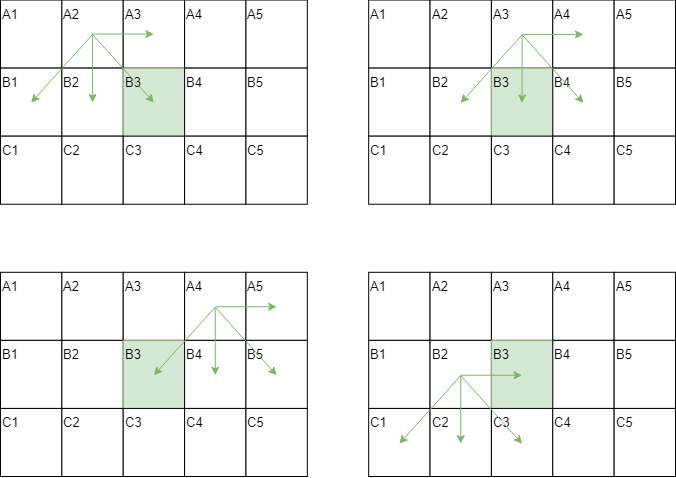
\includegraphics[width=0.5\textwidth]{images/Floyd_process.png}
    \caption{B3 has to wait for pixel calculations from A2, A3, A4 and B2 before it can be worked on}
    \label{fig:process_sketch}
\end{figure}

\noindent If we want to process B3, we have to wait for A2, A3, A4 and B2 to be processed before we can start working. This applies to almost every pixel in the picture except the first row. In the first row, the pixels do not have any restriction in being processed as they only depend on the pixels preceding them on the same row. In our implementation, we divide the image by rows and assign the threads in such a way that each thread takes charge of a single row of pixels. We achieve this with the help of \textit{static scheduling} using OpenMP's \texttt{schedule(static,1)} directive.

\medskip
\noindent Now, as Thread 0 begins processing the first row of pixels, Thread 1 cannot work on its current pixel until Thread 0 moves forward by a sufficient enough distance such that Thread 1's current pixel is completely processed. In this case, Thread 0 will have to be a minimum of 2 spaces ahead of Thread 1 for it to be able to safely work on its current pixel. The same logic can be applied to the subsequent threads working on the image. \textbf{Hence, for a pixel to be considered safe for processing, the pixel one space above and two spaces ahead should be in a completed state}.

\begin{figure}[h]
    \centering
    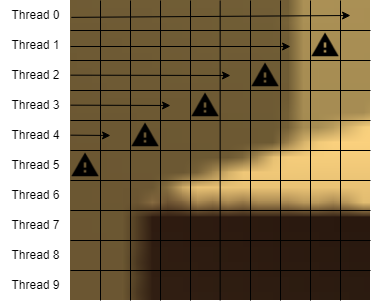
\includegraphics[width=0.4\textwidth]{images/parallel_floyd2.png}
    \caption{A Representation of how the execution order would be}
    \label{fig:cornell_box2}
\end{figure}

\medskip
\noindent The progress marking\cite{Hartley} mechanism of the threads is implemented by using a boolean array with the same dimensions as the given image. Every time a thread completes processing a given pixel, it will update the progress marker at the same coordinates as its current pixel before moving along to the next pixel. This progress tracker is used by subsequent threads in execution blocking.

\medskip
\noindent The execution blocking mechanism for each of the threads is implemented by checking the status of the pixels from the progress marker. An empty while loop is made to run on the given thread until the work on the pixel it is tracking is completed after which it is free to perform the calculations one current pixel.

\medskip
\noindent Coming to the execution of the threads towards the end of the rows, since every thread is constantly tracking the progress of the thread above it ensuring that it is at a minimum of two pixels ahead, when the current thread loops over to the second last and last column, it would be safe for the current pixel to be worked on  as the previous thread has already completed processing its row at this point.

\section{Results and Obsesrvations}

\noindent After implementing the parallelized version of this algorithm in our code, we run it on the same test images we used before in section [\ref{Implementing Floyd-Steinberg Dithering}] and make the following initial observations:

\begin{itemize}
    \item Processing a small test image of 512x512 dimensions on 1 thread takes, on average, 0.189 seconds.

    \item Processing a small test image of 512x512 dimensions on 12 threads takes, on average, 0.127 seconds.

    \item Processing a large test image of 7680x4320 dimensions on 1 thread takes, on average, 21.675  seconds.

    \item Processing a large test image of 7680x4320 dimensions on 12 threads takes, on average, 14.322 seconds.
\end{itemize}

\medskip
\noindent We then perform a strong scaling test with the same images used in section [\ref{Implementing Floyd-Steinberg Dithering}]. The results for the strong scaling tests are shown on the next page [Fig.\ref{fig:scaling_tests}]. We would ideally also perform weak scaling tests on our algorithm, however, to be able to do so, we would need to find a set of quantifiable images with pixel resolutions that would scale accordingly with the number of threads being used, and also in such a way that the workload taken by each thread scales up evenly. I tried searching for, and even creating these images myself, but was unable to do so.

\begin{figure}[H]
    \centering
    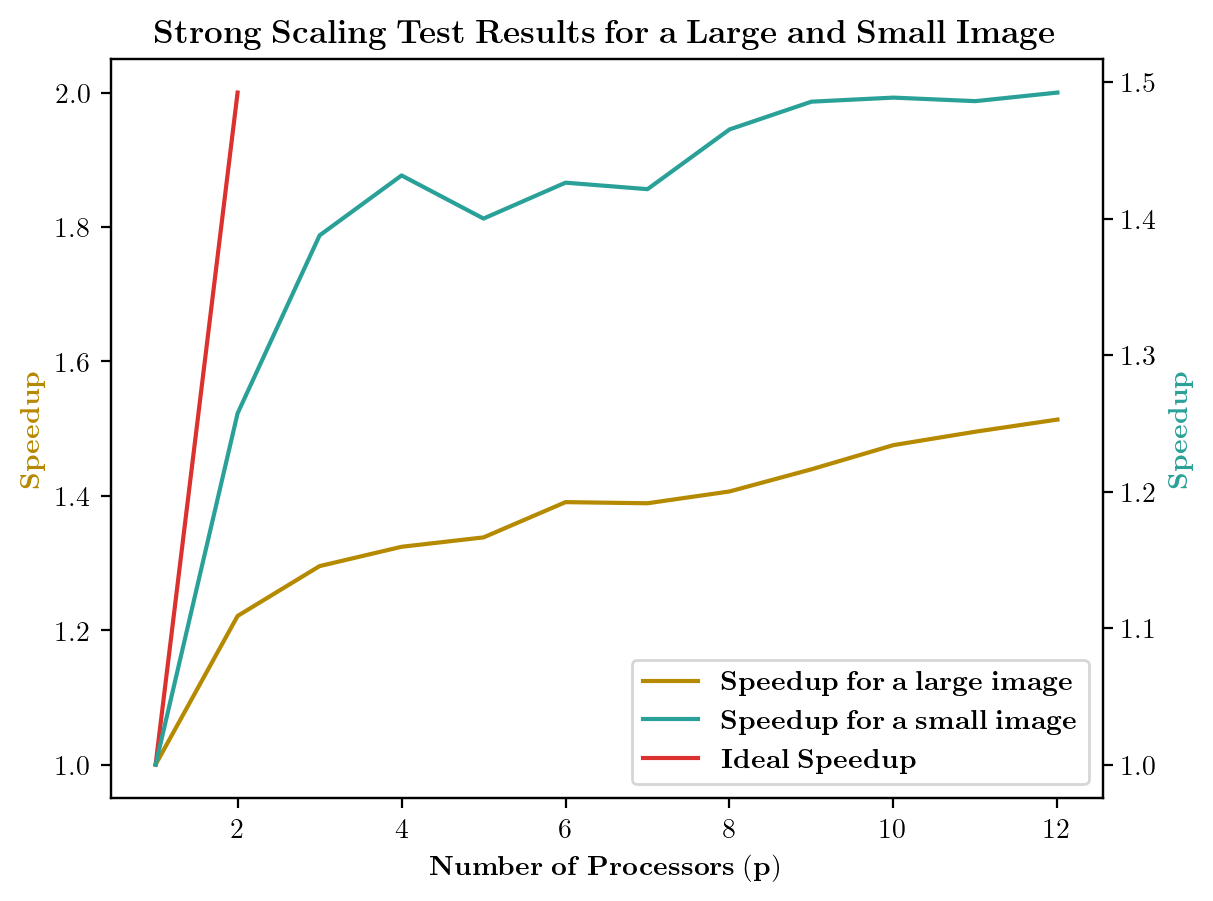
\includegraphics[width=0.55\textwidth]{graphs/strong_scaling_test_plots.png}
    \caption{Strong Scaling Tests for a Small (512x512px) and Large (7680x4320px) Image}
    \label{fig:scaling_tests}
\end{figure}

\noindent We observe that, for a single thread, our program takes more than double the amount of time needed to process the same image in serial. As we increase the number of threads, we see some improvement in the speedup, but it reaches a saturation point after just 2 threads and then begins to plateau while approaching 12 threads. Even at 12 threads, our code was unable to process the images at faster times than our serial code.

\medskip
\noindent To confirm that our parallelized dithering algorithm gives the same output as the serial version of the same, we use a 100x100 pixel test image and run it through the serial and parallel versions of the code. Due to the size of this image, each of the pixels can easily be distinguished from one another, hence allowing us to visually compare the results of our programs.

\begin{figure}[H]
    \centering
    
\includegraphics[width=0.30\textwidth]{images/RGB_color_gradient_100x100.png}
    \caption{The Original Image}
    \label{fig:confirmation_image}
\end{figure}

\begin{figure}[h]
  \centering
  \begin{subfigure}[t]{0.30\textwidth}
    \centering
    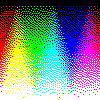
\includegraphics[width=\textwidth]{images/dithered_RGB_color_gradient_100x100.png}
    \caption{Serial Dithering Result}
    \label{fig:serial_dithering_confirmation}
  \end{subfigure}
  ~
  \begin{subfigure}[t]{0.30\textwidth}
    \centering
    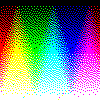
\includegraphics[width=\textwidth]{images/parallel_dithered_RGB_color_gradient_100x100.png}
    \caption{Parallel Dithering Result}
    \label{fig:parallel_dithering_confirmation}
  \end{subfigure}
  \caption{A comparison of the dithering results from our serial and parallel codes.}
\end{figure}

\section{Conclusion and Future Scope}

We were able to successfully implement the Floyd-Steinberg Dithering Algorithm in parallel, and the processed images generated by it are, from what we can observe, highly accurate to the original result from the serial version of the code.

\medskip
\noindent However, as can be seen from the strong scaling test, the performance of the parallel code is much lower than what we would have normally expected. Judging from our approach to parallelizing this algorithm, the processing speed of all the other threads is highly dependent on a single thread's processing speed, i.e. the thread working on the topmost row of pixels. This could have severe implications for the performance of our parallel code.

\medskip
\noindent  In addition, considering the algorithm itself, the calculations being performed are simple, which would reduce its performance in a parallel computing sense. We would see a definite increase in performance if the calculations being done were more complex, such as the handling of complex floating point calculations.

\medskip
\noindent In addition, compared to the serial code which has only a single thread looping over the entire image and performing the calculations, here, each thread has more overhead attributed to it in terms of tracking the value of a boolean array, running a loop and updating the boolean array, all while performing the same calculations that the serial code is doing. These processes, though seemingly small, increase the computational complexity per thread, hence adding to the execution time.

\subsection{Future Scope}

Some interesting things that could be looked into in relation to the future scope of this project are

\begin{itemize}

    \item Finding better approaches to implement this algorithm that could lead to better performance with a little bit of tradeoff on the accuracy of the end result.
    
    \item Implementing this algorithm using GPU-CPU communication\cite{Hartley}. Since GPUs have a high number of cores, it would be intersting to convert this algorithm into a form meant to run on them and study its performance.

    \item Modifying the current algorithm to work on video files.

    \item Studying the memory taken up by the resultant images after dithering. Preliminary tests during the development of the code showed that, for smaller images, the dithered result would take up less space, however, for large images at 1080p and above, the result would take up much more space!

    \item Looking into other noise generation algorithms such as Atkinson Dithering and Perlin Noise.\\ (Fun Fact: Perlin Noise was developed by Ken Perlin after working on the sci-fi motion film Tron(1982)).

\end{itemize}

\printbibliography[title={References}]


\end{document}
